\typeout{ ====================================================================}
\typeout{ this is file main.tex, created at 21-Nov-2014               }
\typeout{ maintained by Gustavo Rabello dos Anjos                             }
\typeout{ e-mail: gustavo.rabello@gmail.com                                   }
\typeout{ ====================================================================}

\documentclass[a4paper,portuges]{article}
\usepackage{babel,varioref,floatflt,wrapfig}
\usepackage{amsmath,booktabs}
\usepackage[utf8]{inputenc}
\usepackage[T1]{fontenc}   % Font Encoding T1 - caracteres acentuados.
\usepackage[top=2cm,bottom=2cm,left=2cm,right=2cm]{geometry}
\usepackage{graphicx}    % pacote para inclusao de figuras,
\usepackage{subfig}
%\pagestyle{empty}
\newcommand{\HRule}{\rule{\linewidth}{0.5mm}}

%%%%%%%%%%%%%%%%%%%%%%%%%%%%%  MACROS MATEMATICOS %%%%%%%%%%%%%%%%%%%%%%%%%%%%%
\newcommand{\tr}{{\,\rm tr}\,}
\newcommand{\sen}{{\,\rm sen}\,}
\newcommand{\senh}{{\,\rm senh}\,}
\newcommand{\diverg}{{\,\rm div}\,}
\newcommand{\grad}{\,\mathbf{grad}\,}
\newcommand{\rot}{\,\mathbf{rot}\,}
\newcommand{\uvet}{\mathbf{u}}
\newcommand{\vvet}{\mathbf{v}}
\newcommand{\wvet}{\mathbf{w}}
\newcommand{\cvet}{\mathbf{c}}
\newcommand{\xvet}{\mathbf{x}}
\newcommand{\gvet}{\mathbf{g}}
\newcommand{\fvet}{\mathbf{f}}
\newcommand{\nvet}{\mathbf{n}}
\newcommand{\tvet}{\mathbf{t}}
\newcommand{\Imat}{\mathbf{I}}
\newcommand{\Eo}{\mathrm{Eo}}
\newcommand{\N}{\mathrm{N}}
\newcommand{\Mo}{\mathrm{Mo}}
%%%%%%%%%%%%%%%%%%%%%%%%%%%%%  MACROS MATEMATICOS %%%%%%%%%%%%%%%%%%%%%%%%%%%%%
										    
\begin{document}	
\typeout{ ====================================================================}
\typeout{ this is file title.tex, created at 21-Nov-2014               }
\typeout{ maintained by Gustavo Rabello dos Anjos                             }
\typeout{ e-mail: gustavo.rabello@gmail.com                                   }
\typeout{ ====================================================================}

\begin{titlepage}
\begin{center}

% Upper part of the page. The '~' is needed because \\
% only works if a paragraph has started.

\includegraphics[width=0.2\textwidth]{./figs/uerj.png}~\\[1cm]

\includegraphics[width=0.3\textwidth]{./figs/gesar.png}~\\[1cm]

\textsc{\LARGE Universidade do Estado do Rio de Janeiro}\\[1.5cm]

\textsc{\Large Relatório Parcial de Atividades -- CAPES}\\[0.5cm]

% Title
\HRule \\[0.4cm]
{ \huge \bfseries Sistema de Simulação Numérica de Escoamentos
Multifásicos\\[0.4cm] }
{ \Large \bfseries Projeto: A067/2013\\[0.4cm] }
\HRule \\[1.0cm]

% Author and supervisor
\noindent
\large
\emph{Bolsista Jovem Talento:}\\
Gustavo R. \textsc{Anjos}\\
\vspace{0.3cm}
\emph{Coordenador:}\\
Norberto \textsc{Mangiavacchi}\\
\vfill

% Bottom of the page
{\large \today}

\end{center}
\end{titlepage}

\typeout{ ****************** End of file title.tex ****************** }



\section{Identificação}

\noindent Dados do Coordenador: 
\begin{itemize}
	\item \textbf{Nome:} Norberto Mangiavacchi
	\item \textbf{CPF:} 732.841.227-53
	\item \textbf{Escolaridade:} Doutorado
	\item \textbf{Endereço Profissional:} Rua Fonseca Teles, 121 --
	Prédio Anexo, CEP 20940-903 São Cristóvão, RJ - Rio de Janeiro
	\item \textbf{Telefone Profissional:} +55 21 2332-4733
	\item \textbf{Endereço Eletrônico:} {\tt norberto@uerj.br}, 
	                                    {\tt norberto@uerj.br}
	\item \textbf{Página Profissional:} {\tt http://www.gesar.uerj.br}
\end{itemize}

\hspace{1cm}

\noindent Dados do Bolsista: 
\begin{itemize}
	\item \textbf{Nome:} Gustavo Rabello dos Anjos
	\item \textbf{CPF:} 042.432.587-08
	\item \textbf{Escolaridade:} Doutorado
	\item \textbf{Endereço Profissional:} Rua Fonseca Teles, 121 --
	Prédio Anexo, CEP 20940-903 São Cristóvão, RJ - Rio de Janeiro
	\item \textbf{Telefone Profissional:} +55 21 2332-4733
	\item \textbf{Endereço Eletrônico:} {\tt gustavo.anjos@uerj.br}
	\item \textbf{Página Profissional:} {\tt http://www.gesar.uerj.br}
	\item \textbf{Página Pessoal:} {\tt http://gustavo.rabello.org}
\end{itemize}

\clearpage

\section{Resumo}
Após um ano completo do projeto CAPES - Bolsa de Atração de Jovens
Talentos, os objetivos e metas previstos para o primeiros período foram
realizados com sucesso. Este documento descreve os resultados obtidos
pelo pesquisador bolsista Gustavo Rabello dos Anjos no projeto
entitulado "Sistema de Simulação Numérica de Escoamentos Multifásicos". 
\clearpage

\section{Introdução}
Deseja-se abordar o desenvolvimento e o estudo numérico de dois
problemas atuais como continuidade de projetos de pesquisa e
desenvolvimento realizados na Universidade do Estado do Rio de
Janeiro/GESAR: 

\begin{itemize}
\item Sistema de simulação numérica de produção, estocagem,
transporte e consumo de metano da decomposição de biomassa em
reservatórios de hidrelétricas (Edital FAPERJ 09/2013 – Programa de
apoio às engenharias 2013); 
\item Simulação numérica de estrutura de
não-equilíbrio em sistemas químicos, biológico e ambientais (Edital de
Cooperação Internacional – Chamada Bilateral CNPq 17/2013 – Bélgica).
\end{itemize}

Ambos com suporte técnico-científico do simulador de escoamentos
multifásicos escrito em linguagem orientada a objetos (MATLAB/C++)
utilizando moderna discretização das equações de governo através do
método de elementos finitos. Para execução do projeto proposto,
planeja-se concluir o desenvolvimento do simulador para modelos
tridimensionais e axisimétricos através da incorporação das seguintes
características: paralelização dos núcleos de cálculo intensivo em
clusters baseados em processadores de vários núcleos (multicore),
extensa validação do modelo numérico através de validações analíticas e
experimentais, este último com colaboração internacional, e publicação
dos resultados em canais de comunicação internacionais de excelência.
Com isso, objetiva-se o aperfeiçoamento das técnicas computacionais
empregadas na instituição de execução do projeto (UERJ/GESAR),
consolidando o Programa de Pós-graduação em Engenharia Mecânica na UERJ,
e a formação de recusos humanos, com aperfeiçoamento pessoal de nível
superior e pós-graduação. Os indicadores de desempenho que serão
utilizados no projeto estão baseados em publicações produzidas pelo
bolsista na UERJ, juntamente com o aluno envolvido na bolsa de IC, e
submetidos a avaliações da comunidade científica.

\section{Objetivos}
\begin{itemize}
	\item estudo e desenvolvimento de modelo em três dimensões e axisimétrico
	      para escoamentos multifásicos;
	\item estudo de escoamentos multifásicos com ondas capilares em bolhas
	      submetidas a campo de temperatura variável;
	\item realização de experimentos computacionais e laboratoriais de
		  decomposição de biomassa e produção de gases com sedimentação
		  de material orgânico; de medição da sedimentação/ressuspensão
		  e consumo de produtos;
	\item validação dos modelos desenvolvidos para sistemas existentes com
	      utilização de tecnologia de última geração;
	\item estudo e desenvolvimento de modelos tridimensionais e axisimétricos
		  para simulação numérica de estrutura de não-equilíbrio em
		  sistemas químicos, biológico e ambientais;
	\item incorporação das seguintes características ao simulador numérico:
		  paralelisação dos núcleos de cálculo intensivo em clusters
		  baseados em processadores de vários núcleos (multicore),
		  através do desenvolvimento de novos precondicionadores para a
		  aceleração dos métodos iterativos implantados e validação do
		  modelo proposto através de soluções analíticas e experimentais
		  (com participação de universidades internacionais);
	\item publicação de resultados em canais de comunicação nacionais e
	      internacionais renomados.
\end{itemize}

\section{Metodologia}
Nesta seção, detalharemos a metodologia utilizada no desenvolvimento do
simulador numérico de escoamentos multifásicos. Para tal, subdiviremos
as seções pela temática da metodogia, a saber: Equações de Governo,
Método de Elementos Finitos, Discretização do Termo de Tensão
Superficial e Solução do Sistema Linear.

\subsection{Equações de Governo}
O princípio de conservação de massa estabelece que, dado um fluido
qualquer com massa específica $\rho$ que escoa através de um volume de
controle V invariante no tempo, a taxa de acumulação de massa no
interior do volume é igual ao fluxo líquido de massa para fora do
volume, em módulo. Para o problema proposto neste trabalho, onde não há
variação da massa específica do fluido em cada fase, ou seja, a massa
específica é constante em cada fase, a equação de conservação de massa
representada em coordenadas cartesianas para 3 dimensões é escrita como:

\begin{equation}
	\frac{\partial v_x}{\partial x} +
	\frac{\partial v_y}{\partial y} +
	\frac{\partial v_z}{\partial z}  
	= 
	0
	\label{eq:cm9}
\end{equation}

Para obtenção das equações de conservação da quantidade de movimento
linear para fluidos newtonianos realiza-se o mesmo procedimento de
obtenção da equação de conservação de massa. O princípio de conservação
da quantidade de movimento estabelece que, dado um fluido qualquer com
massa escoa específica $\rho$ que escoa através de um volume de controle
V, a taxa de acumulação de quantidade de movimento é igual ao fluxo
líquido de quantidade de movimento para fora do volume mais a resultante
das forças de superfície e de volume. A equação de conservação de
quantidade de movimento linear representada em coordenadas cartesianas é
dada por:

\begin{equation}
	\frac{D \vvet}{D t} = - \frac{1}{\rho} \nabla p +
	\frac{1}{\mu} \nabla \cdot [\nu(\nabla \vvet + \nabla \vvet^T)] + 
	\textbf{g} + 
	\textbf{f}
\label{eq:NS3a}
\end{equation}

O princípio do transporte de energia estabelece que, dado um
fluido qualquer com massa específica $\rho$ que escoa através de um
volume de controle V, a taxa de acumulação da quantidade de energia
que entra no volume por unidade de tempo é igual ao fluxo
líquido de massa para fora do volume, na ausência de termos relacionados
ao trabalho e a dissipação toma a forma final representada em
coordeandas cartesianas como:

\begin{equation}
	\frac{DT}{Dt} =  \nabla \cdot (k \nabla T)
\label{eq:quimica2}
\end{equation}\vspace{0.5cm}


	\begin{equation}
		\frac{\partial \vvet}{\partial t} + \vvet \cdot \nabla \vvet
		=
		-\frac{1}{\rho} \nabla p + \frac{1}{Re} \nabla \cdot
		[\nu ( \nabla \vvet + \nabla \vvet^T)]+
		\frac{1}{Fr^2} \mathbf{g} + 
		\frac{1}{We} \mathbf{f}
		\label{eq:final1}
	\end{equation}
	\begin{equation}
		\diverg \cdot \vvet = 0
		\label{eq:final2} 
	\end{equation}	
	\begin{equation}
		\frac{\partial T}{\partial t} + \vvet \cdot \nabla T
		=
		\frac{1}{RePr} \nabla \cdot (k \nabla T)
		\label{eq:final3}
	\end{equation}\vspace{0.5cm}

Para solução do problema de escoamentos multifásicos, procuramos então
encontrar a solução dos campos de velocidade $\vvet$, pressão $p$ e
temperatura $T$ enunciados nos três princípios de conservação descritos
acima. Como a solução analítica destas equações são restritas a
pouquíssmimos casos práticos, onde muitas simplificações são realizadas,
utilizamos uma metodologia numérica de aproximação de solução para
encontramos os valores dos campos $\vvet$, $p$ e $T$ em geometrias
complexas que são pertinentes ao projeto proposto. 

\subsection{Método de Elementos Finitos}
Nos anos 50, o método de elementos finitos teve grande utilização na
mecânica de sólidos.  Apenas a partir da década de 70, após a
consolidação do método de Galerkin para equações de difusão,
pesquisadores começaram a investir no campo da dinâmica dos fluidos,
pode-se citar \cite{zienkiewicz1965}, \cite{oden1972}, \cite{oden1998},
\cite{chung1978}, \cite{hughes1982}, \cite{pironneau1989} e tantos
outros.  Em seguida, vários autores contribuíram para o desenvolvimento
de metodologias específicas como métodos de Petrov-Galerkin
generalizados \cite{heinrich1977}, \cite{hughes1986},
\cite{johnson1987}, métodos adaptativos \cite{oden1989}, métodos de
Taylor-Galerkin \cite{donea1984}, \cite{lohner1985}, método de Galerkin
descontínuo \cite{oden1998} etc.

O começo relativamente tardio no campo da Física de fluidos se deve,
principalmente, à presença do termo convectivo e ao forte acoplamento
entre velocidade e pressão, presentes nas equações de conservação. O
termo convectivo apresenta produto de incógnitas, caracterizando a
não-linearidade do problema e gerando operadores não simétricos, de
difícil solução.  Com o aumento do número de \emph{Reynolds}, o termo
convectivo exerce maior influência no escoamento, aumentando ainda mais
a dificuldade de solução das equações.

Outra fonte de dificuldade numérica é a condição de incompressibilidade,
que consiste em manter o campo de velocidade com divergência zero.
Então, a pressão deve ser considerada uma variável não relacionada a
qualquer equação constitutiva.  Sua presença nas equações de conservação
de quantidade de movimento tem o propósito de introduzir um grau de
liberdade a mais necessário para satisfazer a condição de divergência
zero do campo de velocidades.  Isto é, a pressão atua como um
multiplicador de Lagrange na condição de incompressibilidade resultando
em um acoplamento entre velocidade e pressão desconhecidas.

\subsection{Discretização do Termo de Tensão Superficial}

Em códigos do tipo "front-tracking" a construção da interface é feita
através de um conjunto de objetos geométricos, como triângulos,
segmentos de reta e nós, que são movidos na forma de lagrangian, onde a
malha de fundo é fixada no espaço. Uma função adicional é necessária
para comunicação entre as malhas, uma vez que não há nenhuma
interconectividade implícita. esta abordagem mantém a interface entre as
fases com espessura zero, no qual uma representação precisa é obtida.
Apesar de sua excelente definição geométrica , as propriedades do fluido
perto da interface exigem tratamento numérico para evitar instabilidades
indesejáveis. Como consequência, estas propriedades são suavizados ao
longo da zona de transição e a espessura nula já não pode ser mais
garantida.




Unlike front-tracking codes, the present surface and background meshes
are part of the same computational mesh, thus no additional equation is
required to pass the information from one mesh to another. The
3-dimensional mesh comprises a set of tetrahedron elements distributed
on the domain and the interface is found by a scalar function, namely
Heaviside, which defines the nodes belonging to each phase and the
interface itself. To achieve a zero-thickness representation, the
interface's nodes must be connected consistently so that the piecewise
discrete interface may be represented by a set of interconnected
triangles. In other words, each triangle is a face of two adjacent
tetrahedral elements. Figure~(\ref{fig:inter}a) shows a schematic
representation of the discrete interface between the two different
phases. The same triangle face is shared by two adjacent tetrahedrons,
therefore the zero-thickness interface is successfully achieved.

\begin{figure}[ht!]
		\subfloat[]{
		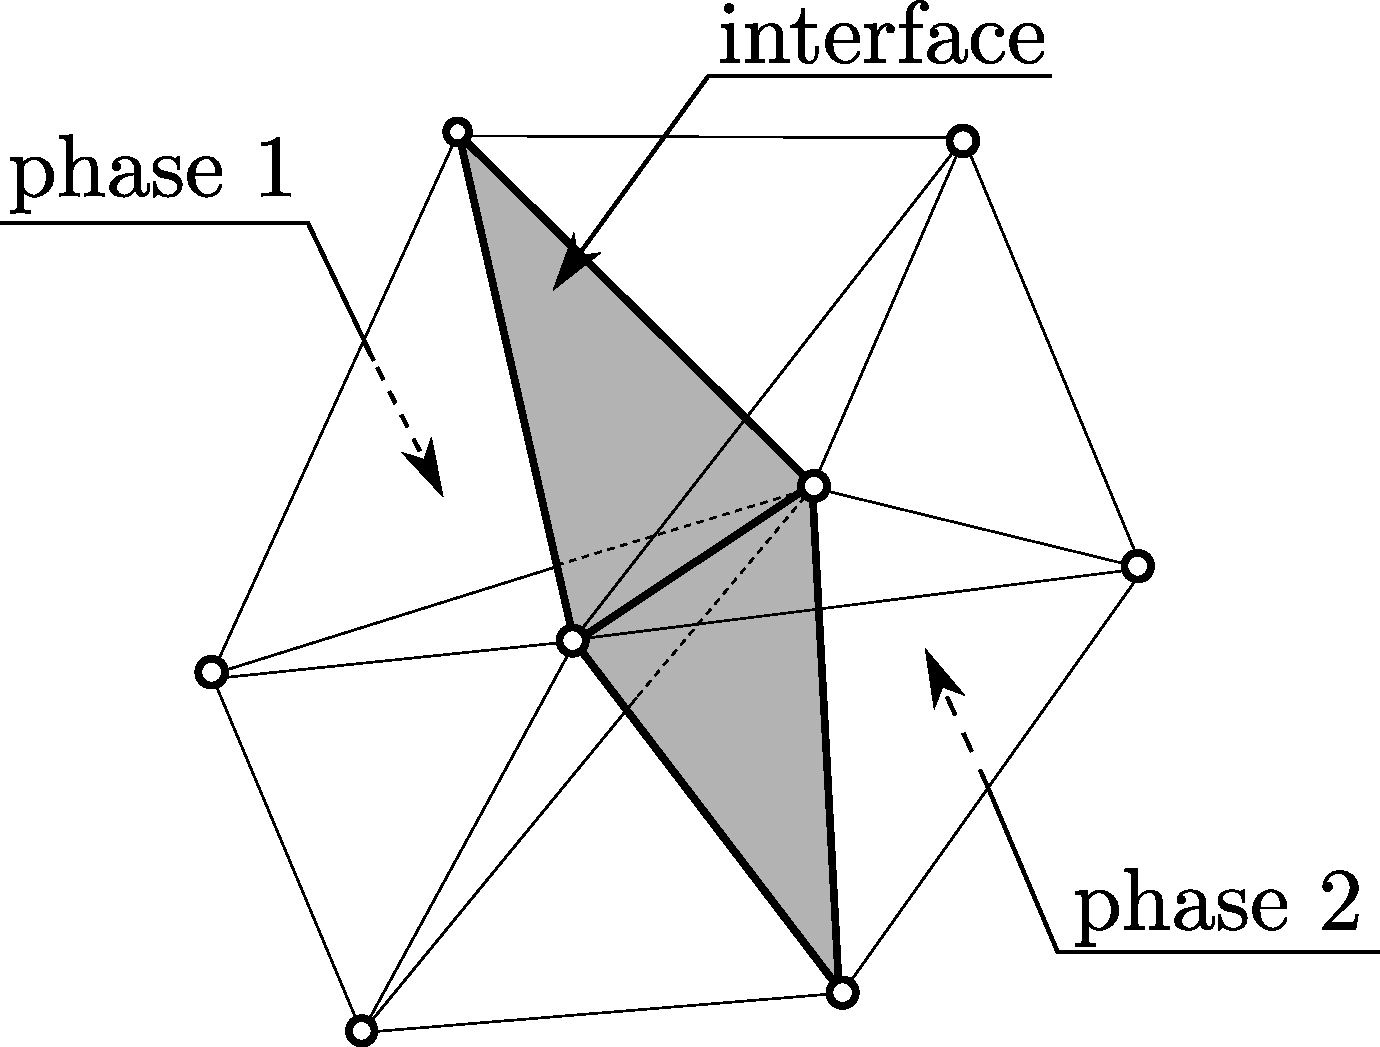
\includegraphics[scale=0.3]{figs/interface.pdf}}
		\subfloat[]{
		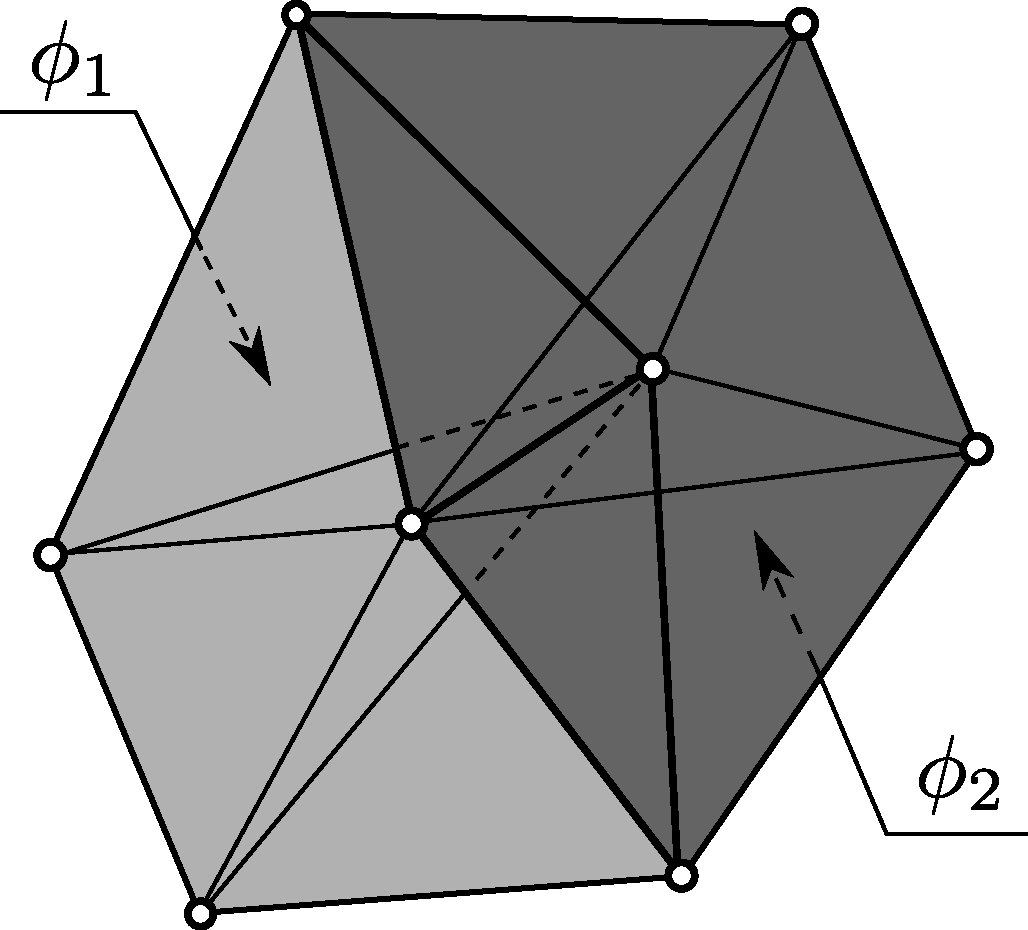
\includegraphics[scale=0.3]{figs/property.pdf}}
	\caption{Geometrical representation of the interface between the
	phases. (a) The interface (gray colored) is represented by a set of
	triangles, edges and nodes which are part of the tetrahedron mesh.
	(b) The fluid property $\phi$, such as density or viscosity, is
	sharply defined in phase $1$ and phase $2$ with a zero thickness
	interface in the transition zone.}
	\label{fig:inter} 
\end{figure}

Advantages and drawbacks are found in such an approach, but one feature
is especially interesting due to the definition of the fluid properties
in the transition area. From the macroscopic point of view, the physical
meaning of an interface is the region that sharply divides the volume
occupied by each phase. Thus, it is desirable that such an interface's
thickness should be kept as thin as possible. The Lagrangian description
guaranties the geometrical part, but due to the abrupt change in
properties from one phase to another, numerical instabilities may appear
and deteriorate the accuracy of the solution. Such a problem is mainly
due to the location of the interface somewhere in-between two
computational elements. This can be circumvented with the ALE and the
Finite Element formulation, in which the interface is not located in
between mesh elements but it shares the faces of two adjacent
computational mesh elements and thus the fluid properties remain
constant in each mesh element. A sharp transition of properties is thus
successfully achieved and does not require the use of any smoothing
functions, consequently assuring accuracy in the balance of forces close
to the interface. 

Figure~(\ref{fig:inter}b) shows the transition zone between the two
phases colored by dark and light gray, which was purposely drawn to
highlight the methodology proposed by this work. As can be seen, the
property $\phi_1$ fills the elements of phase 1 and the property
$\phi_2$ fills exactly the elements of phase 2. Even for a high property
ratio $\phi_1 / \phi_2 = 1000$, the methodology proposed here does not
present spurious oscillation in the pressure and the velocity field.
Figure~(\ref{fig:density}) depicts a 1-dimensional plot of density
distribution along the phases. Figure~(\ref{fig:density}a) shows a the
density distribution used in the implemented ALE-FE scheme. Due to the
Finite Element formulation, each phase property $\phi$ is assigned to
each tetrahedron element, thus a sharp transition of properties is
achieved. Figure~(\ref{fig:density}b) shows a smoothed distribution
commonly found in Level-Set methods. Such a procedure is required to
avoid numerical instabilities close to the interface.

Despite the sharp definition of the interface and the fluid properties,
topological changes are not naturally handled in this method, thus
requiring an implementation effort on the modeling of coalescence and
break-up of bubbles and drops. To address this issue, a geometrical
model may be used to merge or split two surfaces. For instance, when the
film thickness between two bubbles are smaller than a predefined
parameter, the surfaces are connected and coalescence takes place.
Although the topological change occurs, the physical aspects are not
fulfilled. In fact, the mechanisms of bubble coalescence and break-up is
still an open issue and, consequently, a potential field of future
research. 

As seen earlier in this chapter, the calculation of the surface tension
force is based on the gradient of a Heaviside function $\nabla H$.
According to Chapter~(\ref{ch:fem}), a Finite Element formulation for
the given force is achieved by considering the following scheme:


\begin{equation}
	\frac{1}{We}\mathbf{M} \fvet 
	= 
	\frac{1}{We} \mathbf{\Sigma} \mathbf{G} H_{\lambda}
	\label{eq:surfDiscrete}
\end{equation}

In the above equation, $\mathbf{\Sigma}$ is a diagonal matrix with
elements $\sigma \kappa_1, \sigma \kappa_2, \sigma \kappa_3,\cdots,
\sigma \kappa_{NV}$, where $NV$ is the total number of mesh nodes
relative to the pressure field. The matrix $\mathbf{G}$ stands for the
discrete form of the gradient operator $\nabla$ and $H_{\lambda}$ is the
discrete Heaviside function. Finally, Equation~(\ref{eq:surfDiscrete})
can be substituted into the discrete momentum equation
(Eq.~(\ref{eq:ordinarias2})) and the surface tension term calculation
achieved. 

\section{Atividades Desenvolvidas pelo Bolsista JVT e Bolsista IC}

pelo beneficiário da bolsa de Atração de Jovens Talentos: Gustavo Rabello
dos Anjos
\begin{itemize}
\item estudo e desenvolvimento de modelo em três dimensões e axisimétrico
para escoamentos multifásicos;
\item estudo de escoamentos multifásicos com ondas capilares em bolhas
submetidas a campo de temperatura variável;
\item realização de experimentos computacionais e laboratoriais de
decomposição de biomassa e produção de gases com sedimentação de
material orgânico; de medição da sedimentação/ressuspensão e consumo de
produtos;
\item validação dos modelos desenvolvidos para sistemas existentes com
utilização de tecnologia de última geração;
\item estudo e desenvolvimento de modelos tridimensionais e axisimétricos
para simulação numérica de estrutura de não-equilíbrio em sistemas
químicos, biológico e ambientais;
\item incorporação das seguintes características ao simulador numérico:
paralelisação dos núcleos de cálculo intensivo em clusters baseados em
processadores de vários núcleos (multicore), através do desenvolvimento
de novos precondicionadores para a aceleração dos métodos iterativos
implantados e validação do modelo proposto através de soluções
analíticas e experimentais (com participação de universidades
internacionais);
\item publicação de resultados em canais de comunicação nacionais e
internacionais renomados.
\end{itemize}

Pelo beneficiário da bolsa de Iniciação Científida: Vinícius Augusto Cinquini Mascarenhas
\begin{itemize}
\item Revisão bibliográfica pertinente ao projeto;
\item familiarização com as técnicas desenvolvidas e implementadas no
código numérico;
\item execução de testes no código numérico;
\item aumento da qualificação profissional do aluno de IC através de
desenvolvimento e pesquisa.
\item publicação de trabalho em congresso nacional/internacional.
\end{itemize}

\section{Resultados Obtidos}

\section{Produção Científica}
Abaixo estão listados os artigos publicados em canais de comunicação
internacional em que o pesquisador bolsista teve participação direta.

\begin{itemize}
	\item Finite Element Simulation of Fingering in Convective Dissolution in
	      Porous Media Rachel M. Lucena, Norberto Mangiavacchi, José Pontes,
	      Anne De Wit, Gustavo Anjos, CCIS -- 2014
	\item Comparative CFD Simulations of Gas Transport in Slug Flow from
		  Periodic Arrays with Single or Multiple Bubbles G. P.
		  Oliveira, N. Mangiavacchi, G. Anjosa, J. Pontes, J. R. Thome,
		  CCIS -- 2014.
	\item Topological Remeshing and Locally Supported Smoothing for
	      Bubble Coalescence in Two-Phase Flows
		  Gustavo Charles P. de Oliveira, Norberto Mangiavacchi, Gustavo Anjos
		  John R. Thome, COBEM -- 2013
	\item Finite Element Analysis of Pressure-Driven Laminar Flow Inside
	      Periodically Staggered Arrays
		  Gustavo Charles P. de Oliveira, Gustavo R. Anjos, José Pontes,
		  Norberto Mangiavacchi, CONEM -- 2014
	\item Numerical Simulation of a Periodic Array of bubbles in a
	      channel
	      N. Mangiavacchi, G.C.P. Oliveira, G. Anjos and J. R. Thome,
		  PAMAC -- 2013
	\item A Survey of Results Concerning Steady Solutions and the
	      Stability of a Class of Rotating Flows
		  José Pontes, Norberto Mangiavacchi, Gustavo Rabello dos Anjos,
		  Carlos Mendeza, Rachel Manhães de Lucena, Gustavo C. P.
		  Oliveira and Davi V. A. Ferreira, CCIS -- 2014
\end{itemize}

\section{Plano de Trabalho}
O plano de trabalho proposto para o primeiro período de 4 bimestres de
projeto pode ser encontrado na Fig.(\ref{fig:plano}, juntamente com a
etapa final do projeto. Nota-se que o plano de trabalho foi reduzido em
2 bimestres, pois o pesquisador bolsista foi aprovado no concurso
público para professor adjunto do Departamento de Engenharia Mecânica da
Universidade do Rio de Janeiro, tomando posse no dia 14 de julho de
2014. Em decorrência deste fato, o projeto teve seu prazo reduzido para
final de julho de 2015, totalizando 10 bimestres. 

 \begin{figure}[ht!]
 	\begin{center}
 		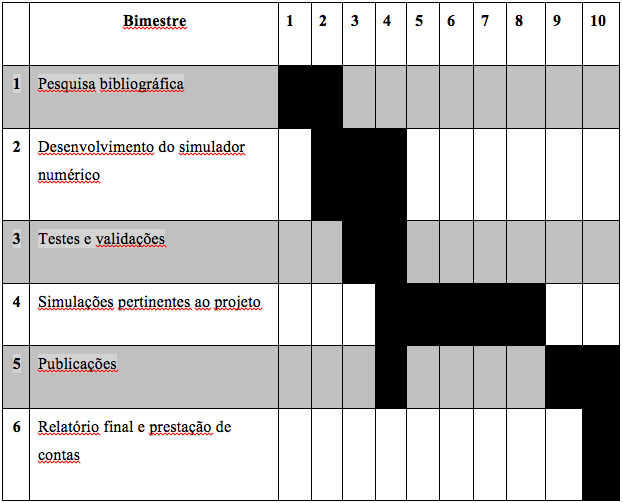
\includegraphics[angle=0, scale=0.5]{figs/plano.png}
 	\end{center}
 	\caption{Plano de trabalho proposto para o período inicial de
	execução do projeto Bolsa de Atração de Jovens Talentos - CAPES.}
 	\label{fig:plano} 
 \end{figure}

A pesquisa bibliográfica foi realizada com sucesso, onde o bolsista
identificou os pontos mais importantes da modelagem matemática e
implementação numérica para realização de sua pesquisa. A partir do 2o.
bimestre foi iniciado o desenvolvimento do simulador numérico, onde
novas funcionalidades foram incorporadas ao já existente código. É
importante notar que o pesquisador bolsista desenvolveu, além de seu
plano de trabalho inicial, um simulador de escoamentos bidimensional em
linguagem de script PYTHON para uso acadêmico, que servirá de apoio nas
aulas ministradas por ele em cursos de graduação e pós-graduação. Alguns
testes e validações foram realizados com sucesso e os resultados podem
ser encontrados na seção de Resultados Obtidos, bem como algumas
simulações pertinentes ao projeto. O pesquisador bolsista participou
ativamente das publicações relacionadas na seção Produção Científica
usando as funcionalidades incorporadas ao simulador através deste
projeto.
\end{document}	

\typeout{ ****************** End of file main.tex ****************** }

